\chapter{Einführung}

\section{Übersicht über die Applikation}

Bei dieser Applikation handelt es sich um ein singleplayer Kartenspiel. 
Hier versucht ein Spieler auf einer einsamen Insel zu überleben und von ihr zu flüchten, 
indem er Karten zieht und Ressourcen (\textit{wood}, \textit{plastic}, \textit{metal}) sammelt, um Gegenstände zu bauen (\textit{Scavange}), 
die ihn vor seinen Feinden (\textit{Encounter}) schützen oder ihm eine Rettung (\textit{Endeavor}) von der Insel ermöglichen. 
Während des Spiels trifft der Spieler auf Tiere (\textit{spider}, \textit{tiger}, \textit{snake}), 
die ihm gesammelte Ressourcen kosten können, oder Katastrophen, 
die Ressourcen zerstören. Das Spiel endet, wenn der Spieler sich retten konnte oder keine Aktionen mehr möglich sind. 

Das Kartenspiel hat verschiedene Spielphasen (s. \autoref{fig:phases}), in denen der Spieler unter bestimmten Bedingungen Karten ziehen 
und Gegenstände bauen kann (\textit{Scavange}). Wenn ein Gegenstand aus der Kategorie Rettungen (\textit{Endeavor}) gebaut wurde, 
muss der Spieler würfeln, um zu entscheiden, ob die Rettung erfolgreich ist. 
Ein Segelboot und ein Hanggleiter stellen eine Rettung dar, 
wenn beim Würfeln eine bestimmte Augenzahl erzielt wird. 
Wenn der Rettungsversuch fehlschlägt, kann der Spieler weiter Karten ziehen und Gegenstände bauen, 
solange Karten im Stapel vorhanden sind. Das Bauen eines Dampfschiffs und eines Heißluftballons 
ist nur mit einer Feuerstelle möglich und garantiert eine erfolgreiche Rettung. Wenn ein Tier gezogen wird, 
muss der Spieler gegen es kämpfen (\textit{Encounter}) und auch hier bestimmt Würfeln über Sieg oder Niederlage.
Für unterschiedliche Aktionen werden unterschiedliche Würfel (\textit{vier-}, \textit{sechs-}, \textit{acht-seitig}) 
verwendet.
Das Spiel endet, wenn keine weiteren Aktionen mehr möglich sind oder wenn eine garantierte Rettung erfolgt ist. 
Wenn das Spiel endet (\textit{End}), bleibt es in diesem Zustand, bis ein neues Spiel gestartet wird, 
bis das Spiel neu initialisiert wird oder die Anwendung beendet wird. 

\begin{figure}
	\centering
	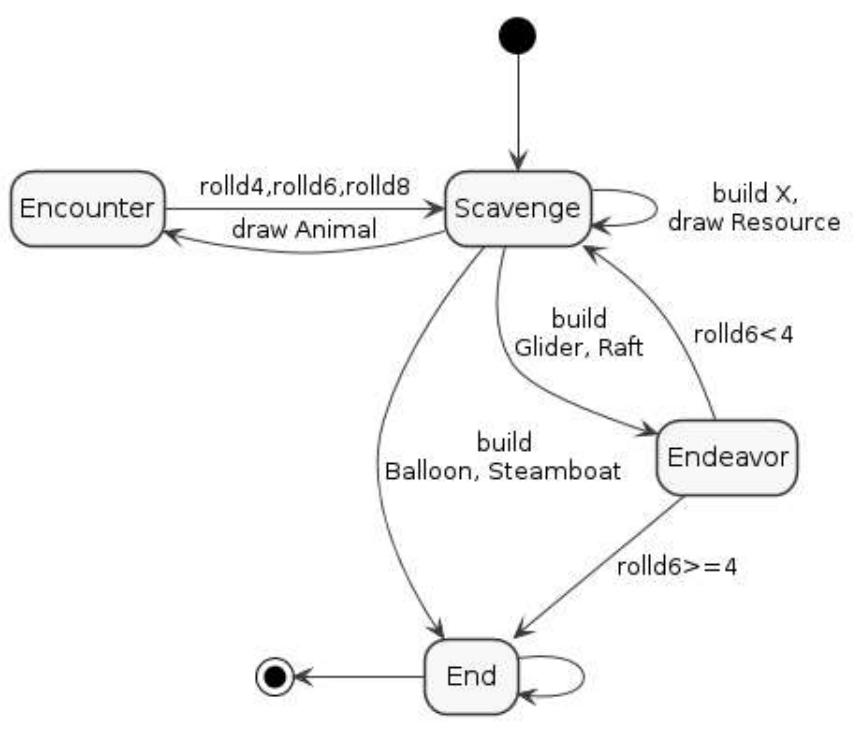
\includegraphics[width=0.6\textwidth]{Bilder/game-phases.png} 
	\caption{Spielphasen.}
	\label{fig:phases}
\end{figure} 

\section{Wie startet man die Applikation?}

Vorraussetzung ist \textbf{Java 17}\footnote{Check mit \texttt{java -version}.}. \\ 
Wahlweise wird eine gängige Java-IDE\footnote{Hier wurde \textit{Jetbrains' IntelliJ} verwendet.} 
\underline{oder} eine \textit{maven}-Installation benötigt.

\subsubsection{Über Maven:} 

Im Wurzelverzeichnis folgende Maven-Befehle ausführen:

\texttt{mvn compile} \\
\texttt{mvn package} \\ 
\texttt{java -jar target/ase-1.0-SNAPSHOT.jar} \\ 
 

\subsubsection{Über IDE:}

Projekt mit IDE im Wurzelverzeichnis öffnen. 
Zu folgendem Pfad navigieren \\ 
\texttt{./src/main/java/de/dhbw/karlsruhe/ase/plugin/cli} \\
und dort die \textit{main}-Methode der Klasse \textit{Main} ausführen lassen.

\subsubsection{Erste Schritte:}

Nun läuft das Command Line Interface der Applikation und es kann mit \\
\texttt{help} \\
eine Übersicht über die möglichen Befehle (Name, Regex, Beschreibung) aufgerufen werden, 
oder mit \\
\texttt{start?} \\
ein Spiel mit zufälligem Kartenstapel gestartet werden. Daraufhin kann mit \\
\texttt{draw} \\
begonnen werden Karten zu ziehen.

\section{Wie testet man die Applikation?}

\subsubsection{Über Maven:}

Im Wurzelverzeichnis:

\texttt{mvn test}

\subsubsection{Über IDE:} 

Die Tests befinden sich unter \\
\texttt{./src/test/java} \\
und können dort mit einer IDE-Funktion ausgeführt werden. \\ 
Es existieren Blackbox-Integration-Tests und Unit-Tests, 
die aber keine besonderen Anforderungen außer eine \textbf{JUnit5}-Abhängigkeit haben.